\documentclass[aspectratio=169]{beamer}


\usetheme{vega}
\renewcommand{\textSupervisors}    {Supervisor}

\title{Forecasting the Yield Curve: An Econometric Study}
\subtitle{}
\author{Vsevolod Zaostrovsky, Ivan Cherepakhin, Artemy Sazonov}
\institute{Lomonosov Moscow State University}
\supervisor{Ivan P. Stankevich}

\begin{document}
\maketitle

\begin{frame}{Data}
    \begin{figure}
        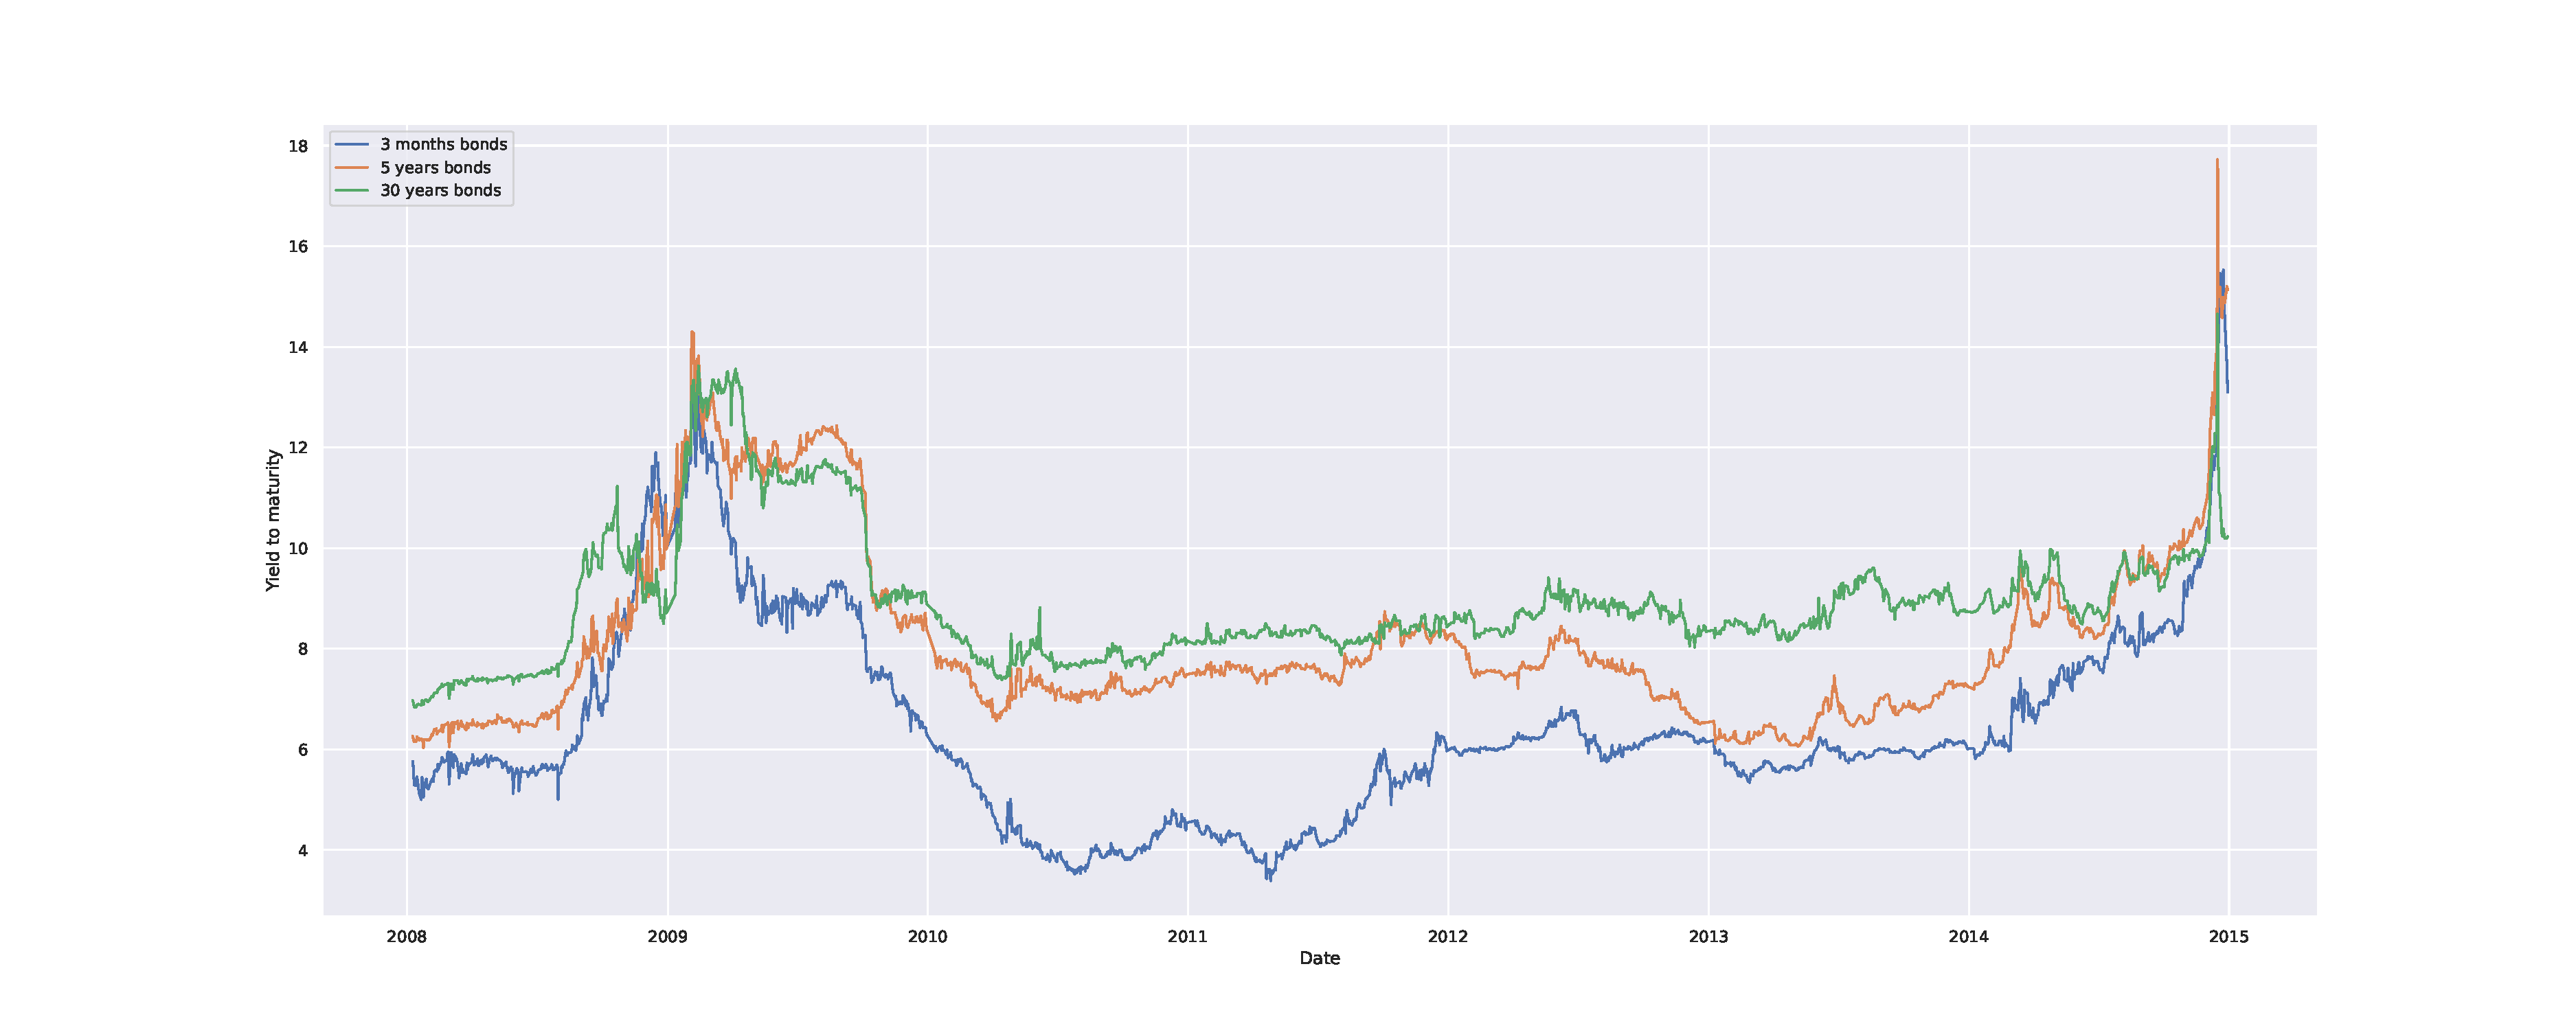
\includegraphics[scale=0.21]{fig/YTMp.pdf}
        \caption{YTM for three different TTM}
        \label{fig:YTMp}
    \end{figure}
\end{frame}

    \begin{frame}{Yield Curve}
        \begin{figure}
            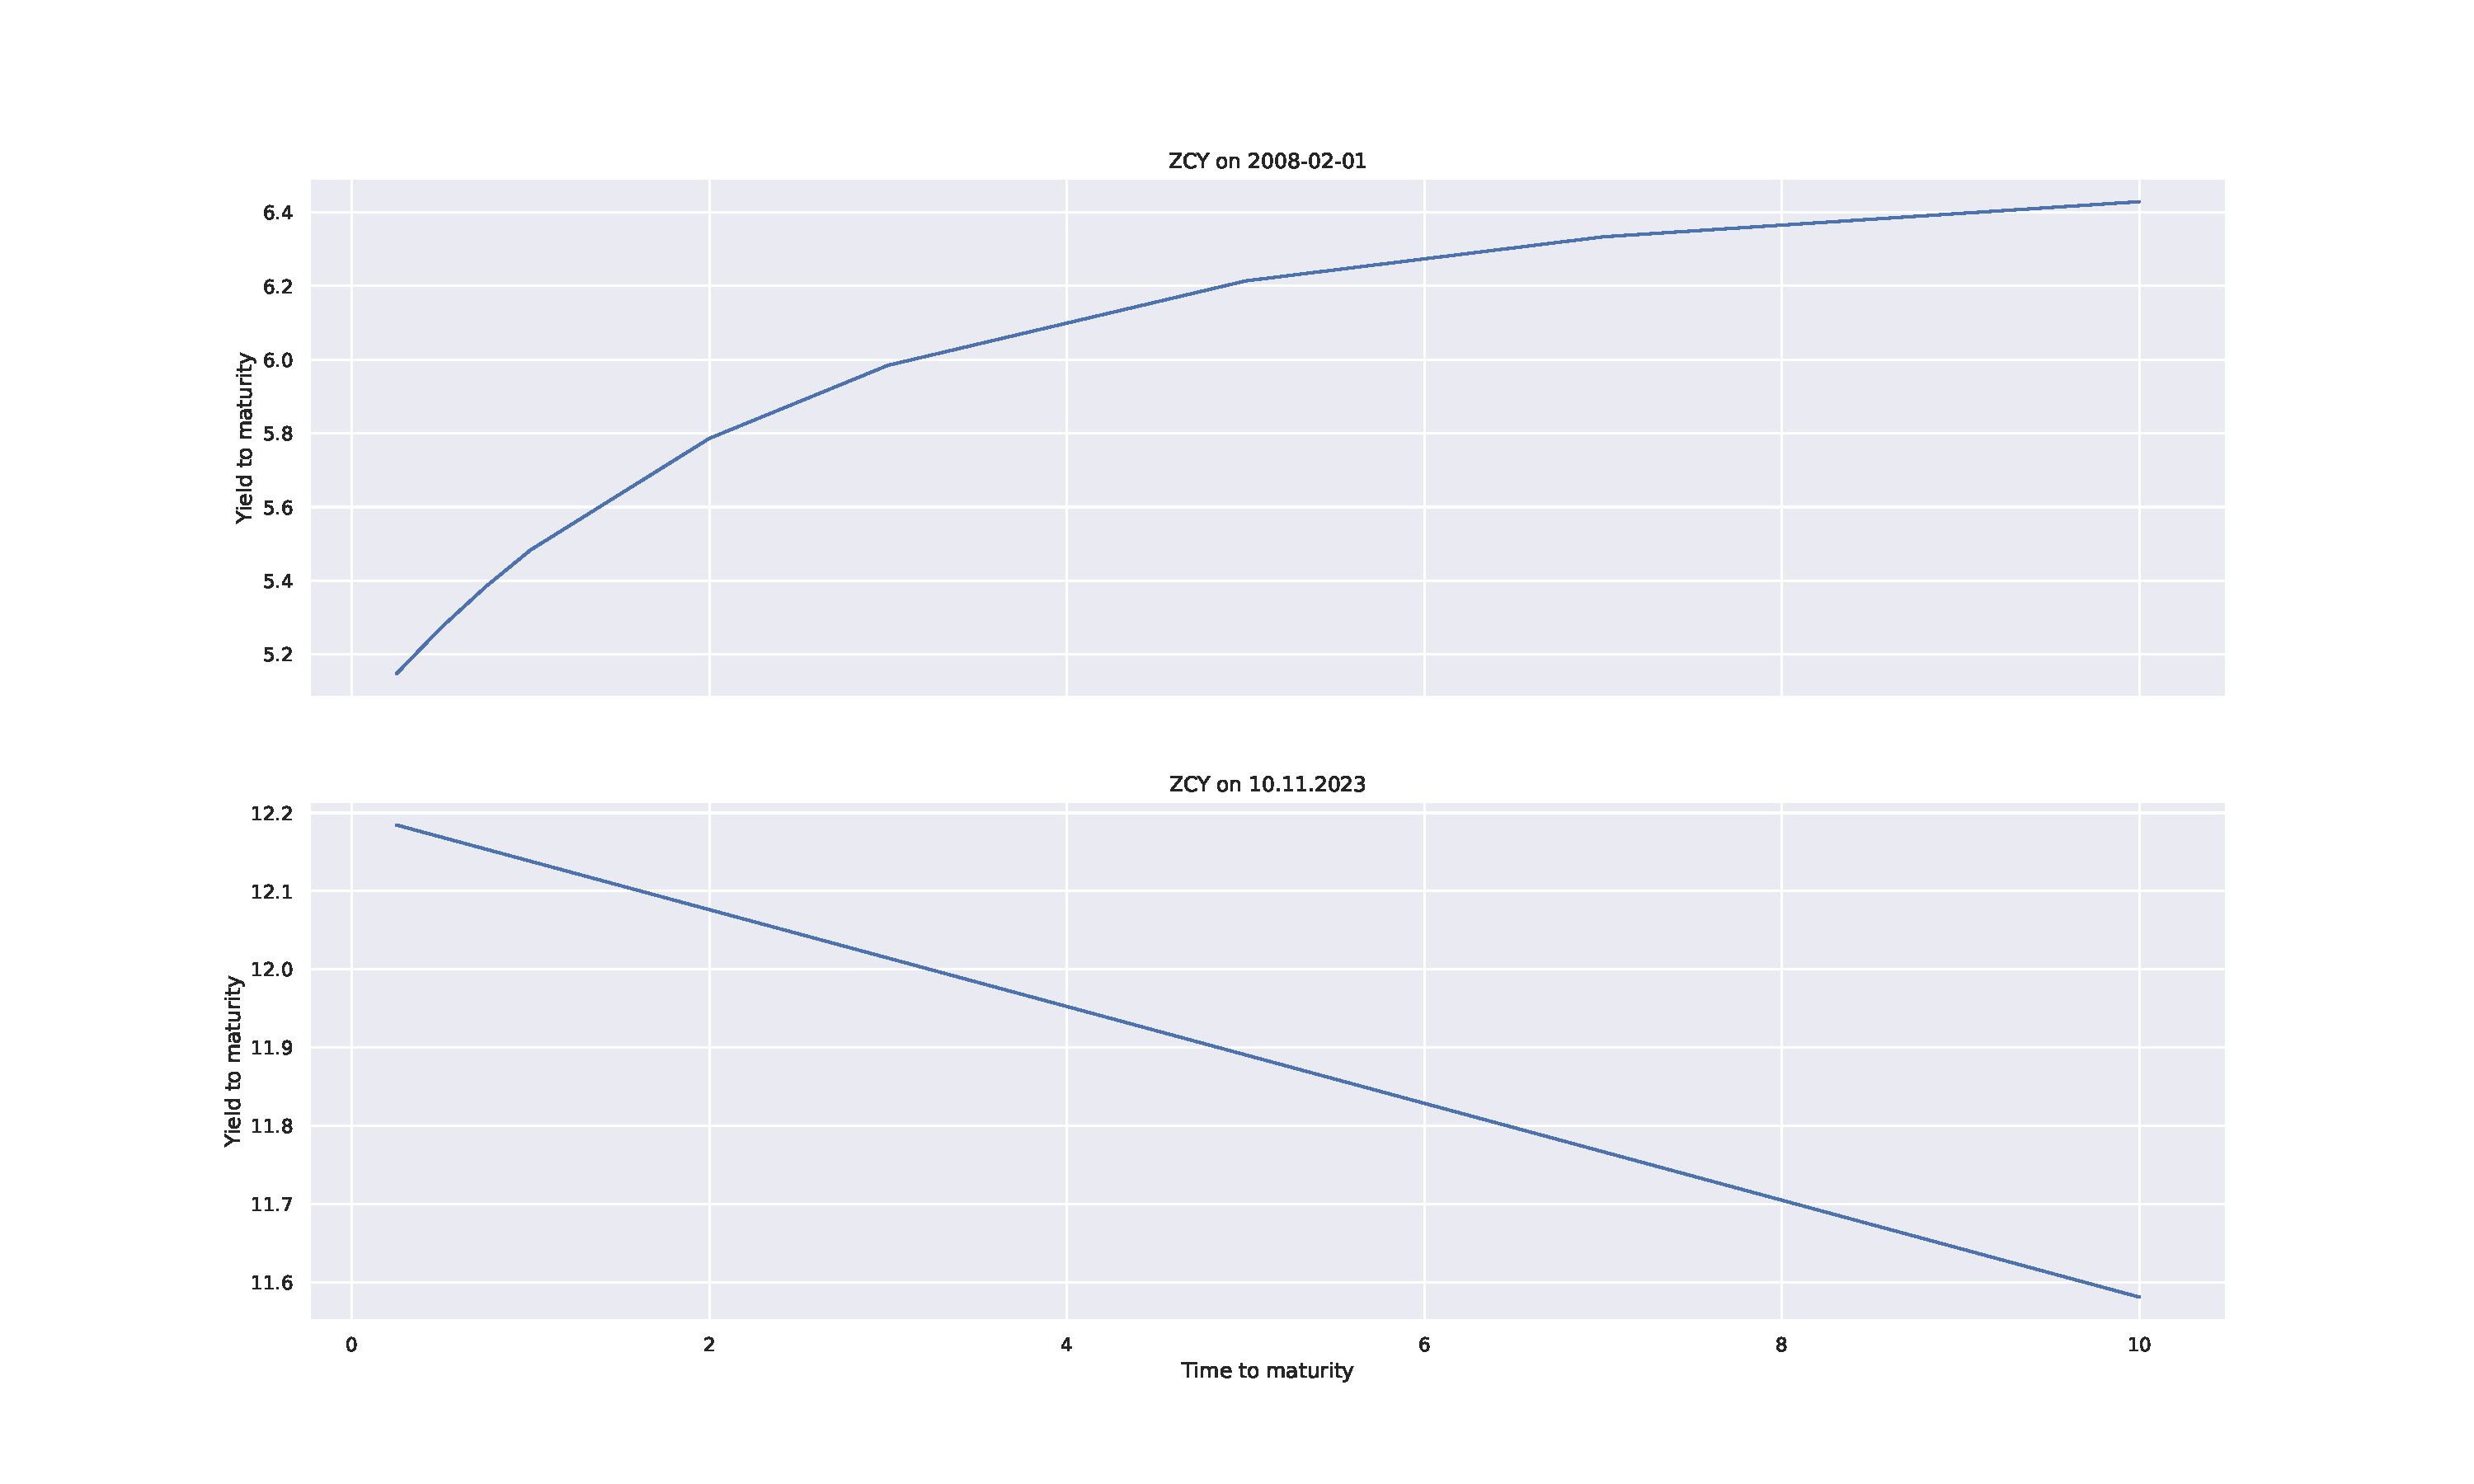
\includegraphics[scale=0.21]{fig/ZCYp.pdf}
            \caption{The yield curves in two different moments of time}
            \label{fig:ZCY}
        \end{figure}
    \end{frame}

    \begin{frame}{Naive approach}{Results (MAE)}
        \begin{table}
            \centering
            \begin{tabular}{|c c c c c c|} 
                \hline
                Time to maturity & auto-ARIMA & ARIMA(0, 0, 0) & RW & VECM(2) & GARCH \\
                \hline
                3m & $0.0045$ & $0.0047$ & $0.0109$ & $0.0193$ & $0.6115$ \\ 
                \hline
                6m & $0.0039$  & 0.$0041$ & $0.0100$ & $0.0182$ & $0.4658$ \\
                \hline
                9m & $0.0035^{**}$ & $0.0038$ & $0.0095$ & $0.0178$ & $0.5676$ \\
                \hline
                12m & $0.0038^{**}$ & $0.0039$ & $0.0069$ & $0.0194$ & $0.7794$ \\
                \hline
                5y & $0.0052$ & $0.0053$ & $0.0072$ & $0.0182$ & $1.2742$\\
                \hline
                15y & $0.0059$ & $0.0061$ & $0.0076$ & $0.0174$ & $1.9276$ \\ 
                \hline
            \end{tabular}
            \caption{}
        \end{table}

    \end{frame}

    \begin{frame}{Nelson-Siegel parametric model}{Model definition}
        The static NS model is defined as follows:
            \begin{equation}\label{eq:NS}
                G(T) = \beta_0 + (\beta_1+\beta_2)\frac{\tau}{T}\left(1-e^{-\frac{T}{\tau}}\right)-\beta_2  e^{-\frac{T}{\tau}},
            \end{equation}
            where $T$ is the time to maturity, $G(T)$ is the yield estimator of the government bonds from the curve basis, 
            and the parameters to be estimated are
            \begin{enumerate}
                \item $\tau$ is the 'typical' time to maturity, 
                \item $\beta_0$ is the long-run of zero-bond yields, 
                \item $\beta_1$ is the mid-run of zero-bond yields, 
                \item $\beta_2$ is the short-run of zero-bond yields.
            \end{enumerate}
    \end{frame}

    \begin{frame}{Nelson-Siegel parametric model}{Forecasting the factors}
        \begin{table}
            \centering
            \begin{tabular}{|c | c c c|} 
                \hline
                Factor & auto-ARIMA & VAR(1) & RW \\
                \hline
                $\beta_0$ & $53.78356$ & $131.1459$ & $66.3105$ \\ 
                \hline
                $\beta_1$ & $63.31042$ & $143.9235$ & $66.25878$ \\
                \hline
                $\beta_2$ & $133.9688$ & $388.3436$ & $177.1525$ \\
                \hline
                $\tau$ & $1.083687$ & $2.569167$ & $1.328986$ \\
                \hline
            \end{tabular}
            \caption{Calibrated factors}
        \end{table}
\end{frame}

    \begin{frame}{Conclusion}
    We found out that:
    \begin{enumerate}
        \item It is better not to use naive time series models to predict bond yields directly \ldots
        \item \ldots since the first difference of bond yields is a <<martingale>> wrt the given information.
        \item Research structural breaks of the yield curve.
    \end{enumerate}
    Our plans for the future of this paper:
    \begin{enumerate}
        \item Try more complicated modifications of Nelson-Siegel model.
        \item Add exogeneous variables.
        \item Research the structural breaks.
    \end{enumerate}
    \end{frame}


\end{document}